\documentclass[tikz,border=6pt]{standalone}
\usepackage{stanli} % <-- stanli

\begin{document}
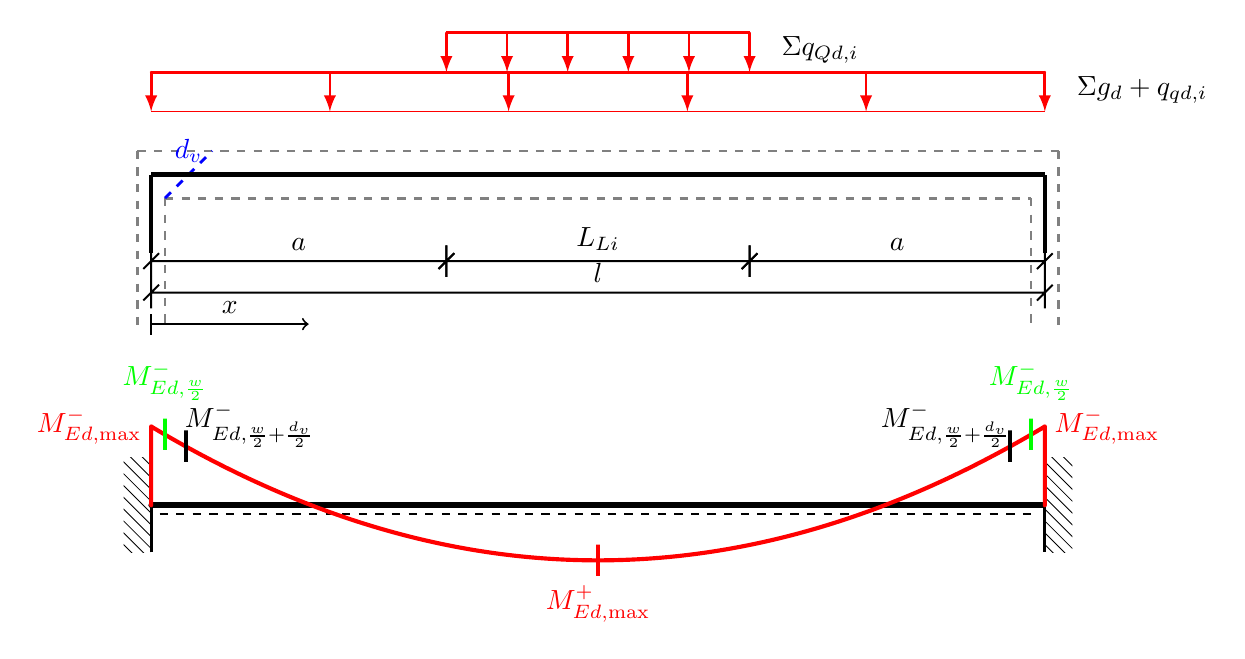
\begin{tikzpicture}

% ============================================================
% 1) SCALA (opzionale, comoda per far stare tutto bene)
% ============================================================
%\scaling{2}; % scala solo le distanze tra i punti (stanli)

% ============================================================
% 2) PUNTI PRINCIPALI (coordinate in "cm" della figura)
% ============================================================
% Trave orizzontale A---B
\point{A}{0}{0};
\point{B}{11.35}{0}; % lunghezza grafica ~ 11.35
\point{A1}{0}{-1};
\point{B1}{11.35}{-1};
% Punti intermedi per indicare a -- L_Li -- a (solo per quote)
\point{A2}{3.75}{0};
\point{B2}{7.60}{0}; % 11.35 - 3.75 = 7.60

%punti per inserire le coordinate
\point{x1}{0}{-1.9}
\point{x2}{2}{-1.9}

% Punti per inserire le due forze
\point{F1}{0}{0.5};
\point{F1e}{11.35}{0.5};
\point{F2}{3.75}{1};
\point{F2e}{7.60}{1};

% Punti del diagramma momento (sotto)
\point{MA}{0}{-4.2};
\point{MB}{11.35}{-4.2};
\point{Mmax}{5.675}{-4.9}
\point{MminA}{0}{-3.2};
\point{MminB}{11.35}{-3.2};
\point{Mw1}{0.175}{-3.3};
\point{Mw2}{11.175}{-3.3};
\point{Mwdv1}{0.445}{-3.45};
\point{Mwdv2}{10.905}{-3.45};

%punti per disegnare la struttura
\point{AngoloAltoSinistra}{-0.175}{0.3}
\point{AngoloAltoDestra}{11.525}{0.3}
\point{AngoloBassoSinistra}{0.175}{-0.3}
\point{AngoloBassoDestra}{11.175}{-0.3}
\point{DiagonaleDv}{0.775}{0.3}

\point{PareteEsternaSinistra}{-0.175}{-2}
\point{PareteEsternaDestra}{11.525}{-2}
\point{PareteInternaSinistra}{0.175}{-1.9}
\point{PareteInternaDestra}{11.175}{-1.9}

% ============================================================
% Sottostruttura tratteggiata
% ============================================================

\begin{scope}[color=gray]
\beam{3}{AngoloAltoSinistra}{AngoloAltoDestra}
\beam{3}{AngoloBassoSinistra}{AngoloBassoDestra}
\beam{3}{AngoloAltoSinistra}{PareteEsternaSinistra}
\beam{3}{AngoloBassoSinistra}{PareteInternaSinistra}
\beam{3}{AngoloAltoDestra}{PareteEsternaDestra}
\beam{3}{AngoloBassoDestra}{PareteInternaDestra}
\end{scope}

\begin{scope}[color=blue]
\beam{3}{AngoloBassoSinistra}{DiagonaleDv}
\notation{1}{DiagonaleDv}{$d_v$}[left]
\end{scope}


% ============================================================
% 3) TRAVE (beam) + INCASTRI (support type 3)
% ============================================================
% beam type 4 = trave senza "fibra caratteristica" (più pulita)
\beam{2}{A}{B};
\beam{2}{A}{A1};
\beam{2}{B1}{B};
% support type 3 = "fixed support" (incastro) (manuale stanli)

\support{3}{MA}[-90];
\support{3}{MB}[90];
% ============================================================
% 4) CARICO DISTRIBUITO
% ============================================================
% lineload type 2 = forze parallele all'asse y (verticali)
% sintassi: \lineload{2}{inizio}{fine}[q_i][q_f][intervallo]
% Se metti q_i=q_f ottieni carico uniforme
\begin{scope}[color=red]
\lineload{1}{F1}{F1e}[0.5][0.5];
\lineload{1}{F2}{F2e}[0.5][0.5];
\end{scope}



% (opzionale) etichetta del carico
\notation{1}{F2e}{$\Sigma q_{Qd,i}$}[above right= 0.4];
\notation{1}{F1e}{$\Sigma g_d + q_{qd,i}$}[above right= 0.4];

% ============================================================
% 5) QUOTE (a - L_Li - a) e l
% ============================================================
% dimensioning type 1 = quota orizzontale
\dimensioning{1}{A}{A2}{-1.1}[$a$];
\dimensioning{1}{A2}{B2}{-1.1}[$L_{Li}$];
\dimensioning{1}{B2}{B}{-1.1}[$a$];
\dimensioning{1}{A}{B}{-1.5}[$l$];
 % coordinata x
 \dimensioning{3}{x1}{x2}{0}[$x$];

% ============================================================
% 6) DIAGRAMMA DEL MOMENTO (sotto)
% ============================================================
% Riga di riferimento sotto
\beam{1}{MA}{MB}[1]

% internalforces: \internalforces{inizio}{fine}{val_i}{val_f}[parabola][colore][pos]
% - val_i, val_f: valori ai bordi (grafici)
% - parabola height: "altezza" della parabola (negativa -> verso il basso)
\internalforces{MA}{MB}{-1}{-1}[-1.7][red];

% etichette momento
\begin{scope}[color=red]
\notation{1}{MminA}{$M^-_{Ed,\max}$}[left];
\notation{1}{MminB}{$M^-_{Ed,\max}$}[right];
\notation{2}{Mmax}{$M^+_{Ed,\max}$}[below=0.2]; % solo indicativa
\end{scope}

\begin{scope}[color=green]
\notation{2}{Mw1}{$M^-_{Ed,\frac{w}{2}}$}[above = 0.3];
\notation{2}{Mw2}{$M^-_{Ed,\frac{w}{2}}$}[above = 0.3];
\end{scope}

\begin{scope}[color=black]
\notation{2}{Mwdv1}{$M^-_{Ed,\frac{w}{2}+\frac{d_v}{2}}$}[above right= -0.2];
\notation{2}{Mwdv2}{$M^-_{Ed,\frac{w}{2}+\frac{d_v}{2}}$}[above left= -0.2];
\end{scope}
\end{tikzpicture}
\end{document}
